% Render only generator-admitted canonical records. The generator has
% already enforced identity, evidence, artwork, rights/provenance, and
% edition-selection gates before these calls reach TeX.
% Generated-record API for the Roman Sanctuary Dictionary.
% This file stores data only. Page design belongs to the dictionary format.
\makeatletter

\newcommand{\RSDClearObjectRecord}{%
  \def\RSDObjectID{}%
  \def\RSDPreferredEnglishName{}%
  \def\RSDLatinHeadword{}%
  \def\RSDAlternateEnglishNames{}%
  \def\RSDAlternateLatinNames{}%
  \def\RSDCategories{}%
  \def\RSDPeriods{}%
  \def\RSDStatuses{}%
  \def\RSDCeremonies{}%
  \def\RSDPresenceLocations{}%
  \def\RSDPresenceContexts{}%
  \def\RSDOrdinaryHandlers{}%
  \def\RSDServerRelation{}%
  \def\RSDConfusableWith{}%
  \def\RSDRelatedObjects{}%
  \def\RSDPronunciationKey{}%
}

\newcommand{\RSDObjectRecord}[3]{%
  \RSDClearObjectRecord
  \def\RSDObjectID{#1}%
  \def\RSDPreferredEnglishName{#2}%
  \def\RSDLatinHeadword{#3}%
}
\newcommand{\RSDObjectAliases}[2]{%
  \def\RSDAlternateEnglishNames{#1}%
  \def\RSDAlternateLatinNames{#2}%
}
\newcommand{\RSDObjectClassification}[4]{%
  \def\RSDCategories{#1}%
  \def\RSDPeriods{#2}%
  \def\RSDStatuses{#3}%
  \def\RSDCeremonies{#4}%
}
\newcommand{\RSDObjectPresence}[2]{%
  \def\RSDPresenceLocations{#1}%
  \def\RSDPresenceContexts{#2}%
}
\newcommand{\RSDObjectHandling}[2]{%
  \def\RSDOrdinaryHandlers{#1}%
  \def\RSDServerRelation{#2}%
}
\newcommand{\RSDObjectRelations}[2]{%
  \def\RSDConfusableWith{#1}%
  \def\RSDRelatedObjects{#2}%
}
\newcommand{\RSDObjectPronunciationKey}[1]{%
  \def\RSDPronunciationKey{#1}%
}

% Consumers redefine these append hooks. The generator calls them in declared
% record order. Arguments remain explicit so records can be validated against
% their TOML source without parsing prose inside TeX.
\providecommand{\RSDClaim}[6]{}
% #1 claim ID, #2 kind, #3 text, #4 evidence state,
% #5 comma-separated source IDs, #6 comma-separated applicable variant IDs

\providecommand{\RSDVariant}[7]{}
% #1 variant ID, #2 English name, #3 Latin name, #4 distinguishing features,
% #5 status, #6 source IDs, #7 artwork IDs

\providecommand{\RSDSourceBinding}[6]{}
% #1 local source ID, #2 canonical binding, #3 locus, #4 role,
% #5 verification state, #6 checked-on date or empty

\providecommand{\RSDArtwork}[7]{}
% #1 artwork ID, #2 view, #3 asset path, #4 review state,
% #5 depicted object IDs, #6 variant ID or empty, #7 scale mode

\providecommand{\RSDAudienceNote}[4]{}
% #1 audience, #2 note text, #3 supporting claim IDs, #4 object ID

\providecommand{\RSDEndObjectRecord}{}

\RSDClearObjectRecord
\makeatother


\newcount\RSDRenderedRecordCount
\RSDRenderedRecordCount=0
\newif\ifRSDArtworkAvailable
\newif\ifRSDSecondArtworkAvailable
\newif\ifRSDStoryHero
\newif\ifRSDStoryTallHero
\newif\ifRSDTallCard
\newif\ifRSDSpacedCard
\newif\ifRSDFieldCard
\newif\ifRSDQuadCard
\newif\ifRSDRelationshipCard
\newif\ifRSDSevenCard
\newif\ifRSDDiagnosticCard
\newif\ifRSDWideCard
\newif\ifRSDPairedCard
\newdimen\RSDCardHeight
\newdimen\RSDCardArtworkFieldHeight
\newdimen\RSDCardGraphicHeight
\RSDStoryHerofalse
\RSDStoryTallHerofalse
\RSDTallCardfalse
\RSDSpacedCardfalse
\RSDFieldCardfalse
\RSDQuadCardfalse
\RSDRelationshipCardfalse
\RSDSevenCardfalse
\RSDDiagnosticCardfalse
\RSDWideCardfalse
\RSDPairedCardfalse
\usetikzlibrary{decorations.pathmorphing}
\tikzset{
  rsd pencil line/.style={
    draw=black!82,
    line width=0.65pt,
    line cap=round,
    line join=round,
    decorate,
    decoration={random steps,segment length=4pt,amplitude=0.28pt}
  }
}
\newcommand{\RSDGenericClosedBook}{%
  \pgfmathsetseed{1962}%
  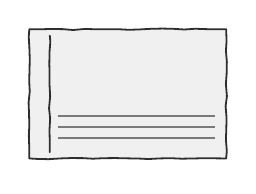
\begin{tikzpicture}[baseline=-0.6ex,x=1cm,y=1cm]
    \fill[black!6] (0,0) rectangle (2.5,1.64);
    \draw[rsd pencil line] (0,0) rectangle (2.5,1.64);
    \draw[rsd pencil line] (0.26,0.08) -- (0.26,1.56);
    \foreach \y in {0.26,0.40,0.54}
      \draw[black!52,line width=0.5pt] (0.36,\y) -- (2.36,\y);
  \end{tikzpicture}}
\newcommand{\RSDGenericOpenBook}{%
  \pgfmathsetseed{1963}%
  
\begin{tikzpicture}[baseline=-0.6ex,x=1cm,y=1cm]
    \fill[black!4] (0,0.20) -- (1.56,0) -- (1.56,1.56) --
      (0,1.76) -- cycle;
    \fill[black!4] (1.56,0) -- (3.12,0.20) -- (3.12,1.76) --
      (1.56,1.56) -- cycle;
    \draw[rsd pencil line] (0,0.20) -- (1.56,0) -- (1.56,1.56) --
      (0,1.76) -- cycle;
    \draw[rsd pencil line] (1.56,0) -- (3.12,0.20) -- (3.12,1.76) --
      (1.56,1.56);
    \foreach \y in {0.46,0.68,0.90,1.12}
      \draw[black!45,line width=0.45pt] (0.28,\y) -- (1.28,\y);
    \foreach \y in {0.46,0.68,0.90,1.12}
      \draw[black!45,line width=0.45pt] (1.84,\y) -- (2.84,\y);
  \end{tikzpicture}}
\renewcommand{\RSDObjectRecord}[3]{%
  \RSDClearObjectRecord
  \def\RSDObjectID{#1}%
  \def\RSDPreferredEnglishName{#2}%
  \def\RSDLatinHeadword{#3}%
  \def\RSDIdentityText{}%
  \def\RSDUseText{}%
  \def\RSDSymbolismText{}%
  \def\RSDArtworkPath{}%
  \def\RSDSecondArtworkPath{}%
  \def\RSDAudienceText{}%
  \def\RSDNoteNumber{}%
  \def\RSDHandlingText{}%
  \def\RSDWarningsText{}%
  \def\RSDLayerKeyText{}%
  \RSDArtworkAvailablefalse
  \RSDSecondArtworkAvailablefalse}

\renewcommand{\RSDClaim}[6]{%
  \ifstrequal{#2}{identity}{\def\RSDIdentityText{#3}}{}%
  \ifstrequal{#2}{liturgical-use}{\def\RSDUseText{#3}}{}%
  \ifstrequal{#2}{ceremonial-presence}{\def\RSDUseText{#3}}{}%
  \ifstrequal{#2}{symbolism}{\def\RSDSymbolismText{#3}}{}}

\newcommand{\RSDRegisterGeneratedArtwork}[1]{%
  \ifRSDArtworkAvailable
    \ifRSDSecondArtworkAvailable\else
      \ifstrequal{\RSDArtworkPath}{#1}{}{%
        \def\RSDSecondArtworkPath{#1}%
        \RSDSecondArtworkAvailabletrue}%
    \fi
  \else
    \def\RSDArtworkPath{#1}%
    \RSDArtworkAvailabletrue
  \fi}

\renewcommand{\RSDArtwork}[8]{%
  % Shared comparisons and compositions retain every canonical evidence link,
  % but the generator assigns their visible rendering to exactly one record.
  \ifdefstring{\RSDObjectID}{#8}{\RSDRegisterGeneratedArtwork{#3}}{}}

\providecommand{\RSDSelectedAudienceNote}[1]{\def\RSDAudienceText{#1}}
\newcommand{\RSDDisplayCaption}[2]{\def\RSDIdentityText{#1}\def\RSDUseText{#2}}
\newcommand{\RSDObjectNoteNumber}[1]{\def\RSDNoteNumber{#1}}
\newcommand{\RSDHandlingWarnings}[1]{\def\RSDWarningsText{#1}}
\newcommand{\RSDSharedLayerKey}{%
  \def\RSDLayerKeyText{%
    {\fontsize{9.2}{12}\selectfont
      \textbf{Shared vesture study}\par\smallskip
      Inside \(\longrightarrow\) outside\par\smallskip
      1. Pontifical tunicle\par
      2. Pontifical dalmatic\par
      3. Chasuble\par\smallskip
      {\fontsize{7.4}{8.6}\selectfont The shared cutaway shows all three layers.\par}}}}
\newcommand{\RSDHandlingCaption}[1]{\def\RSDHandlingText{#1}}
\newcommand{\RSDNoteMark}{%
  \ifx\RSDNoteNumber\empty\else
    \textsuperscript{\hyperlink{rsd-note-\RSDNoteNumber}{\RSDNoteNumber}}%
  \fi}
\newcommand{\RSDCaption}{%
  \ifx\RSDHandlingText\empty\else\textbf{\RSDHandlingText}\enspace\fi
  \RSDIdentityText\ifx\RSDUseText\empty\else\space\RSDUseText\fi
  \ifx\RSDWarningsText\empty\else
    \par\vspace{2pt}\textbf{Care and limits.}\enspace\RSDWarningsText
  \fi}
\newcommand{\RSDPlateFooter}{%
  \par\vfill\noindent\hrule height 0.35pt\vspace{4pt}
  \DictionaryScaleNotice\par}

\newsavebox{\RSDCardTitleBox}
\newcommand{\RSDCardTitle}[1]{%
  \sbox{\RSDCardTitleBox}{\fontsize{9.2}{10.2}\selectfont\bfseries #1\RSDNoteMark}%
  \ifdim\wd\RSDCardTitleBox>0.78\linewidth
    \resizebox{0.78\linewidth}{!}{\usebox{\RSDCardTitleBox}}\par
  \else
    {\raggedright\fontsize{9.2}{10.2}\selectfont\bfseries #1\RSDNoteMark\par}%
  \fi}
\newcommand{\RSDLatinAndKeyLine}[2]{#1\par}

\renewcommand{\RSDEndObjectRecord}{%
  \global\advance\RSDRenderedRecordCount by 1
  \ifRSDStoryTallHero
  \begin{minipage}[t][4.34in][t]{\linewidth}
  \DictionaryEntryAnchor{\RSDObjectID}%
  {\fontsize{14}{15.4}\selectfont\bfseries\RSDPreferredEnglishName\RSDNoteMark\par}
  {\fontsize{8.5}{9.5}\selectfont\itshape
    \RSDLatinAndKeyLine{\RSDLatinHeadword}{\RSDObjectID}}
  \vspace{2pt}\hrule height 0.45pt\vspace{5pt}
  \begin{minipage}[t][3.60in][c]{0.58\linewidth}
    \centering
    \ifRSDArtworkAvailable
      \DictionaryGraphic{3.48in}{liturgy/roman-rite/1962/reference/roman-sanctuary-dictionary/\RSDArtworkPath}
    \else\RSDLayerKeyText
    \fi
  \end{minipage}\hfill
  \begin{minipage}[t][3.60in][t]{0.38\linewidth}
    {\fontsize{8.5}{10}\selectfont
      \RSDCaption\par}
    \ifx\RSDAudienceText\empty\else
      \vspace{5pt}{\fontsize{7.8}{9.2}\selectfont
        \textbf{Look for.}\enspace\RSDAudienceText\par}
    \fi
    \ifx\RSDSymbolismText\empty\else
      \vspace{5pt}{\fontsize{7.6}{9}\selectfont\itshape\RSDSymbolismText\par}
    \fi
  \end{minipage}
  \end{minipage}%
  \global\RSDStoryTallHerofalse
  \else\ifRSDStoryHero
  \begin{minipage}[t][3.06in][t]{\linewidth}
  \DictionaryEntryAnchor{\RSDObjectID}%
  {\fontsize{13}{14.2}\selectfont\bfseries\RSDPreferredEnglishName\RSDNoteMark\par}
  {\fontsize{8.2}{9.2}\selectfont\itshape
    \RSDLatinAndKeyLine{\RSDLatinHeadword}{\RSDObjectID}}
  \vspace{2pt}\hrule height 0.45pt\vspace{4pt}
  \begin{minipage}[t][2.40in][c]{0.49\linewidth}
    \centering
    \ifRSDArtworkAvailable
      \DictionaryGraphic{2.34in}{liturgy/roman-rite/1962/reference/roman-sanctuary-dictionary/\RSDArtworkPath}
    \else\RSDLayerKeyText
    \fi
  \end{minipage}\hfill
  \begin{minipage}[t][2.40in][t]{0.47\linewidth}
    {\fontsize{8.2}{9.6}\selectfont
      \RSDCaption\par}
    \ifx\RSDAudienceText\empty\else
      \vspace{4pt}{\fontsize{7.5}{8.8}\selectfont
        \textbf{Look for.}\enspace\RSDAudienceText\par}
    \fi
    \ifx\RSDSymbolismText\empty\else
      \vspace{4pt}{\fontsize{7.3}{8.5}\selectfont\itshape\RSDSymbolismText\par}
    \fi
  \end{minipage}
  \end{minipage}%
  \global\RSDStoryHerofalse
  \else\ifRSDTallCard
  \begin{minipage}[t][6.72in][t]{\linewidth}
  \DictionaryEntryAnchor{\RSDObjectID}%
  {\fontsize{11}{12.2}\selectfont\bfseries\RSDPreferredEnglishName\RSDNoteMark\par}
  {\fontsize{7.7}{8.7}\selectfont\itshape
    \RSDLatinAndKeyLine{\RSDLatinHeadword}{\RSDObjectID}}
  \vspace{2pt}\hrule height 0.4pt\vspace{4pt}
  \begin{minipage}[t][4.12in][c]{\linewidth}
    \centering
    \ifRSDArtworkAvailable
      \DictionaryGraphic{4.00in}{liturgy/roman-rite/1962/reference/roman-sanctuary-dictionary/\RSDArtworkPath}
    \else\RSDLayerKeyText
    \fi
  \end{minipage}\par
  \vspace{0.30in}
  {\fontsize{7.4}{8.7}\selectfont\raggedright
    \RSDCaption\par}
  \ifx\RSDAudienceText\empty\else
    \vspace{4pt}{\fontsize{7}{8.2}\selectfont
      \textbf{Reader note.}\enspace\RSDAudienceText\par}
  \fi
  \ifx\RSDSymbolismText\empty\else
    \vspace{4pt}{\fontsize{6.8}{8}\selectfont\itshape\RSDSymbolismText\par}
  \fi
  \end{minipage}%
  \global\RSDTallCardfalse
  \else
  \ifRSDPairedCard
    \RSDCardHeight=6.72in
    \RSDCardArtworkFieldHeight=4.12in
    \RSDCardGraphicHeight=4.00in
  \else\ifRSDSevenCard
    \RSDCardHeight=4.25in
    \RSDCardArtworkFieldHeight=1.50in
    \RSDCardGraphicHeight=1.44in
  \else\ifRSDDiagnosticCard
    \RSDCardHeight=4.05in
    \RSDCardArtworkFieldHeight=1.82in
    \RSDCardGraphicHeight=1.76in
  \else\ifRSDWideCard
    \RSDCardHeight=3.40in
    \RSDCardArtworkFieldHeight=1.78in
    \RSDCardGraphicHeight=1.72in
  \else\ifRSDRelationshipCard
    \RSDCardHeight=3.18in
    \RSDCardArtworkFieldHeight=1.66in
    \RSDCardGraphicHeight=1.60in
  \else\ifRSDQuadCard
    \RSDCardHeight=3.60in
    \RSDCardArtworkFieldHeight=1.94in
    \RSDCardGraphicHeight=1.88in
  \else\ifRSDFieldCard
    \RSDCardHeight=4.05in
    \RSDCardArtworkFieldHeight=1.56in
    \RSDCardGraphicHeight=1.50in
  \else
    \RSDCardHeight=3.90in
    \RSDCardArtworkFieldHeight=1.54in
    \RSDCardGraphicHeight=1.48in
  \fi\fi\fi\fi\fi\fi\fi
  \begin{minipage}[t][\RSDCardHeight][t]{\linewidth}
  \DictionaryEntryAnchor{\RSDObjectID}%
  \RSDCardTitle{\RSDPreferredEnglishName}
  {\fontsize{7.1}{8}\selectfont\itshape
    \RSDLatinAndKeyLine{\RSDLatinHeadword}{\RSDObjectID}}
  \vspace{2pt}\hrule height 0.35pt\vspace{3pt}
  \begin{minipage}[t][\RSDCardArtworkFieldHeight][c]{\linewidth}
    \centering
    \ifRSDArtworkAvailable
      \ifRSDSecondArtworkAvailable
        \begin{minipage}[c]{0.48\linewidth}\centering
          \ifRSDPairedCard
            \DictionaryGraphic{3.90in}{liturgy/roman-rite/1962/reference/roman-sanctuary-dictionary/\RSDArtworkPath}
          \else
            \DictionaryGraphic{1.08in}{liturgy/roman-rite/1962/reference/roman-sanctuary-dictionary/\RSDArtworkPath}
          \fi
          \ifdefstring{\RSDObjectID}{obj-cassock}{%
            \par{\fontsize{7}{8}\selectfont\bfseries Cassock alone}}{}
          \ifdefstring{\RSDObjectID}{obj-altar-cruet}{%
            \par{\fontsize{6}{6.8}\selectfont\bfseries One cruet}}{}
          \ifdefstring{\RSDObjectID}{obj-epistle-book}{%
            \par{\fontsize{6}{6.8}\selectfont\bfseries The book itself}}{}
          \ifdefstring{\RSDObjectID}{obj-gospel-book}{%
            \par{\fontsize{6}{6.8}\selectfont\bfseries The book itself}}{}
        \end{minipage}\hfill
        \begin{minipage}[c]{0.48\linewidth}\centering
          \ifRSDPairedCard
            \DictionaryGraphic{3.90in}{liturgy/roman-rite/1962/reference/roman-sanctuary-dictionary/\RSDSecondArtworkPath}
          \else
            \DictionaryGraphic{1.08in}{liturgy/roman-rite/1962/reference/roman-sanctuary-dictionary/\RSDSecondArtworkPath}
          \fi
          \ifdefstring{\RSDObjectID}{obj-cassock}{%
            \par{\fontsize{7}{8}\selectfont\bfseries Cassock with surplice}}{}
          \ifdefstring{\RSDObjectID}{obj-altar-cruet}{%
            \par{\fontsize{6}{6.8}\selectfont\bfseries Wine-and-water pair}}{}
          \ifdefstring{\RSDObjectID}{obj-epistle-book}{%
            \par{\fontsize{6}{6.8}\selectfont\bfseries Carried context}}{}
          \ifdefstring{\RSDObjectID}{obj-gospel-book}{%
            \par{\fontsize{6}{6.8}\selectfont\bfseries Sung context}}{}
        \end{minipage}
      \else
        \ifdefstring{\RSDObjectID}{obj-processional-cross}{%
          \includegraphics[height=1.45in,keepaspectratio]{%
            liturgy/roman-rite/1962/reference/roman-sanctuary-dictionary/\RSDArtworkPath}%
        }{%
          \DictionaryGraphic{\RSDCardGraphicHeight}{liturgy/roman-rite/1962/reference/roman-sanctuary-dictionary/\RSDArtworkPath}%
        }%
      \fi
    \else\RSDLayerKeyText\fi
  \end{minipage}\par
  \ifRSDSpacedCard\vfill\else\vspace{3pt}\fi
  {\fontsize{7.4}{8.6}\selectfont\raggedright
    \RSDCaption\par}
  \ifx\RSDAudienceText\empty\else
    \vspace{2pt}{\fontsize{7}{8.1}\selectfont\raggedright
      \textbf{Reader note.}\enspace\RSDAudienceText\par}
  \fi
  \ifx\RSDSymbolismText\empty\else
    \vspace{2pt}{\fontsize{6.1}{7}\selectfont\itshape\RSDSymbolismText\par}
  \fi
  \end{minipage}%
  \global\RSDSpacedCardfalse
  \global\RSDFieldCardfalse
  \global\RSDQuadCardfalse
  \global\RSDRelationshipCardfalse
  \global\RSDSevenCardfalse
  \global\RSDDiagnosticCardfalse
  \global\RSDWideCardfalse
  \global\RSDPairedCardfalse
  \fi\fi\fi}

\newcommand{\RSDDensePlateStart}[2]{%
  \clearpage
  {\fontsize{8}{9}\selectfont\bfseries\MakeUppercase{Comparison plate}
    \hfill #1\enspace\textperiodcentered\enspace #2\par}
  \vspace{2pt}\hrule height 0.65pt\vspace{6pt}
  % The asymmetric widths create a stable visual lead and supporting pair.
  % The second row mirrors that hierarchy instead of repeating a card grid.
  \noindent\begin{tabular}{@{}p{0.37\textwidth}@{\hspace{0.025\textwidth}}%
    p{0.275\textwidth}@{\hspace{0.025\textwidth}}p{0.305\textwidth}@{}}}
\newcommand{\RSDDensePlateCellBreak}{&}
\newcommand{\RSDDensePlateRowBreak}{%
  \end{tabular}\par\vspace{0.30in}
  \noindent\begin{tabular}{@{}p{0.305\textwidth}@{\hspace{0.025\textwidth}}%
    p{0.275\textwidth}@{\hspace{0.025\textwidth}}p{0.37\textwidth}@{}}}
\newcommand{\RSDDensePlateEnd}{%
  \end{tabular}\par\vfill
  \DictionaryScaleNotice}

% Five-object fields use a three-over-two rhythm. The wider lower pair fills
% the page without suggesting a missing sixth object.
\newcommand{\RSDHeterodoxFivePlateStart}[2]{%
  \clearpage
  {\fontsize{8}{9}\selectfont\bfseries\MakeUppercase{Visual field}
    \hfill #1\enspace\textperiodcentered\enspace #2\par}
  \vspace{2pt}\hrule height 0.65pt\vspace{6pt}
  \noindent\begin{tabular}{@{}p{0.37\textwidth}@{\hspace{0.025\textwidth}}%
    p{0.275\textwidth}@{\hspace{0.025\textwidth}}p{0.305\textwidth}@{}}}
\newcommand{\RSDHeterodoxFivePlateCellBreak}{&}
\newcommand{\RSDHeterodoxFivePlateRowBreak}{%
  \end{tabular}\par\vspace{0.20in}
  \noindent\begin{tabular}{@{}p{0.475\textwidth}@{\hspace{0.05\textwidth}}%
    p{0.475\textwidth}@{}}}
\newcommand{\RSDHeterodoxFivePlateEnd}{%
  \end{tabular}\par\vfill
  \DictionaryScaleNotice}

% Seven-object fields use a four-plus-three rhythm. The centered second row
% keeps the last three studies prominent without duplicating an empty cell.
\newcommand{\RSDDenseSevenPlateStart}[2]{%
  \clearpage
  \noindent
  \begin{minipage}[t]{0.28\textwidth}
    {\fontsize{8}{9}\selectfont\bfseries\MakeUppercase{Working set}\par}
  \end{minipage}\hfill
  \begin{minipage}[t]{0.68\textwidth}
    \raggedleft
    {\fontsize{8}{9}\selectfont\bfseries
      #1\enspace\textperiodcentered\enspace PLATE~#2\par}
  \end{minipage}
  \par\vspace{3pt}\hrule height 0.65pt\vspace{8pt}
  \noindent\begin{tabular}{@{}p{0.235\textwidth}@{\hspace{0.02\textwidth}}%
    p{0.235\textwidth}@{\hspace{0.02\textwidth}}%
    p{0.235\textwidth}@{\hspace{0.02\textwidth}}p{0.235\textwidth}@{}}}
\newcommand{\RSDDenseSevenPlateCellBreak}{&}
\newcommand{\RSDDenseSevenPlateRowBreak}{%
  \end{tabular}\par\vspace{0.18in}
  \noindent\hfill\begin{tabular}{@{}p{0.29\textwidth}@{\hspace{0.025\textwidth}}%
    p{0.29\textwidth}@{\hspace{0.025\textwidth}}p{0.29\textwidth}@{}}}
\newcommand{\RSDDenseSevenPlateEnd}{%
  \end{tabular}\hfill\null\par\vfill
  \DictionaryScaleNotice}

% Four-object comparisons use a balanced two-by-two field. The wider cards
% provide longer labels and reader notes with more breathing room than the
% three-column dense grid while retaining a full visual page.
\newcommand{\RSDBalancedFourPlateStart}[2]{%
  \clearpage
  \noindent
  \begin{minipage}[t]{0.32\textwidth}
    {\fontsize{8}{9}\selectfont\bfseries\MakeUppercase{Comparison plate}\par}
  \end{minipage}\hfill
  \begin{minipage}[t]{0.64\textwidth}
    \raggedleft
    {\fontsize{8}{9}\selectfont\bfseries
      #1\enspace\textperiodcentered\enspace #2\par}
  \end{minipage}
  \par\vspace{3pt}\hrule height 0.65pt\vspace{7pt}
  \noindent\begin{tabular}{@{}p{0.475\textwidth}@{\hspace{0.05\textwidth}}%
    p{0.475\textwidth}@{}}}
\newcommand{\RSDBalancedFourPlateCellBreak}{&}
\newcommand{\RSDBalancedFourPlateRowBreak}{%
  \\[10pt]}
\newcommand{\RSDBalancedFourFilledPlateRowBreak}{%
  \\[0.25in]}
\newcommand{\RSDBalancedFourPlateEnd}{%
  \end{tabular}\par\vfill
  \DictionaryScaleNotice}
\newcommand{\RSDBalancedFourFilledPlateEnd}{%
  \end{tabular}\par\vfill
  \DictionaryScaleNotice}

% Three-object comparisons use two paired studies followed by one centered
% study. This preserves generous diagnostic scale without leaving an accidental
% empty fourth-card hole in a two-by-two field.
\newcommand{\RSDBalancedThreePlateStart}[2]{%
  \clearpage
  {\fontsize{8}{9}\selectfont\bfseries\MakeUppercase{Comparison plate}
    \hfill #1\enspace\textperiodcentered\enspace #2\par}
  \vspace{2pt}\hrule height 0.65pt\vspace{7pt}
  \noindent\begin{tabular}{@{}p{0.475\textwidth}@{\hspace{0.05\textwidth}}%
    p{0.475\textwidth}@{}}}
\newcommand{\RSDBalancedThreePlateCellBreak}{&}
\newcommand{\RSDBalancedThreePlateLastStart}{%
  \end{tabular}\par\vspace{10pt}\noindent\hfill
  \begin{minipage}[t]{0.475\textwidth}}
\newcommand{\RSDBalancedThreePlateEnd}{%
  \end{minipage}\hfill\null\RSDPlateFooter}

% Tall two- and three-object fields use the page height for large recognition
% studies instead of leaving the unused cells of a dense grid visible.
\newcommand{\RSDTallCardNext}{\global\RSDTallCardtrue}
\newcommand{\RSDPairedCardNext}{\global\RSDPairedCardtrue}
\newcommand{\RSDSpacedCardNext}{\global\RSDSpacedCardtrue}
\newcommand{\RSDFieldCardNext}{%
  \global\RSDFieldCardtrue
  \global\RSDSpacedCardtrue}
\newcommand{\RSDQuadCardNext}{%
  \global\RSDQuadCardtrue
  \global\RSDSpacedCardtrue}
\newcommand{\RSDRelationshipCardNext}{%
  \global\RSDRelationshipCardtrue
  \global\RSDSpacedCardtrue}
\newcommand{\RSDSevenCardNext}{\global\RSDSevenCardtrue}
\newcommand{\RSDDiagnosticCardNext}{%
  \global\RSDDiagnosticCardtrue
  \global\RSDSpacedCardtrue}
\newcommand{\RSDWideCardNext}{%
  \global\RSDWideCardtrue
  \global\RSDSpacedCardtrue}
\newcommand{\RSDBalancedTwoTallPlateStart}[2]{%
  \clearpage
  {\fontsize{8}{9}\selectfont\bfseries\MakeUppercase{Relationship study}
    \hfill #1\enspace\textperiodcentered\enspace PLATE~#2\par}
  \vspace{2pt}\hrule height 0.65pt\vspace{7pt}
  \noindent\begin{tabular}{@{}p{0.475\textwidth}@{\hspace{0.05\textwidth}}%
    p{0.475\textwidth}@{}}}
\newcommand{\RSDBalancedTwoTallPlateCellBreak}{&}
\newcommand{\RSDBalancedTwoTallPlateEnd}{%
  \end{tabular}\par\vfill
  \DictionaryScaleNotice}
\newcommand{\RSDBalancedThreeTallPlateStart}[2]{%
  \clearpage
  {\fontsize{8}{9}\selectfont\bfseries\MakeUppercase{Relationship study}
    \hfill #1\enspace\textperiodcentered\enspace PLATE~#2\par}
  \vspace{2pt}\hrule height 0.65pt\vspace{7pt}
  \noindent\begin{tabular}{@{}p{0.31\textwidth}@{\hspace{0.035\textwidth}}%
    p{0.31\textwidth}@{\hspace{0.035\textwidth}}p{0.31\textwidth}@{}}}
\newcommand{\RSDBalancedThreeTallPlateCellBreak}{&}
\newcommand{\RSDBalancedThreeTallPlateEnd}{%
  \end{tabular}\par\vfill
  \DictionaryScaleNotice}
\newcommand{\RSDRelationshipThreePlateStart}[2]{%
  \clearpage
  {\fontsize{8}{9}\selectfont\bfseries\MakeUppercase{Relationship study}
    \hfill #1\enspace\textperiodcentered\enspace PLATE~#2\par}
  \vspace{2pt}\hrule height 0.65pt\vspace{7pt}
  \noindent\begin{tabular}{@{}p{0.31\textwidth}@{\hspace{0.035\textwidth}}%
    p{0.655\textwidth}@{}}}
\newcommand{\RSDRelationshipThreePlateCellBreak}{%
  &\begin{minipage}[t]{\linewidth}}
\newcommand{\RSDRelationshipThreePlateRightBreak}{%
  \par\vspace{8pt}}
\newcommand{\RSDRelationshipThreePlateEnd}{%
  \end{minipage}\end{tabular}\par\vfill
  \DictionaryScaleNotice}

% A story spread varies scale without changing canonical records. One hero
% introduces the group; up to four compact comparison cards follow below.
\newcommand{\RSDStoryPlateStart}[2]{%
  \clearpage
  {\fontsize{8}{9}\selectfont\bfseries\MakeUppercase{Visual field guide}
    \hfill #1\enspace\textperiodcentered\enspace #2\par}
  \vspace{2pt}\hrule height 0.65pt\vspace{6pt}}
\newcommand{\RSDStoryHeroNext}{\global\RSDStoryHerotrue}
\newcommand{\RSDStoryCompanionsStart}{%
  \par\vspace{5pt}\noindent
  \begin{tabular}{@{}p{0.235\textwidth}@{\hspace{0.02\textwidth}}%
    p{0.235\textwidth}@{\hspace{0.02\textwidth}}%
    p{0.235\textwidth}@{\hspace{0.02\textwidth}}p{0.235\textwidth}@{}}}
\newcommand{\RSDStoryCompanionBreak}{&}
\newcommand{\RSDStoryCompanionsEnd}{\end{tabular}\par}
\newcommand{\RSDStoryPlateEnd}{\RSDPlateFooter}

% The tall story archetype gives one vertically distinctive object a full
% field, then closes with three related recognition cards across the foot.
\newcommand{\RSDStoryTallPlateStart}[2]{%
  \clearpage
  {\fontsize{8}{9}\selectfont\bfseries\MakeUppercase{Visual field guide}
    \hfill #1\enspace\textperiodcentered\enspace #2\par}
  \vspace{2pt}\hrule height 0.65pt\vspace{6pt}}
\newcommand{\RSDStoryTallHeroNext}{\global\RSDStoryTallHerotrue}
\newcommand{\RSDStoryTallCompanionsStart}{%
  \par\vspace{4pt}\noindent
  \begin{tabular}{@{}p{0.31\textwidth}@{\hspace{0.035\textwidth}}%
    p{0.31\textwidth}@{\hspace{0.035\textwidth}}p{0.31\textwidth}@{}}}
\newcommand{\RSDStoryTallCompanionBreak}{&}
\newcommand{\RSDStoryTallCompanionsEnd}{\end{tabular}\par}
\newcommand{\RSDStoryTallPlateEnd}{\RSDPlateFooter}

\newcommand{\RSDRenderGeneratedEdition}[1]{%
  \InputIfFileExists{#1}{}{%
    \PackageError{roman-sanctuary-dictionary}
      {Generated edition data not found: #1}
      {Run tools/tpt render-sanctuary-dictionary before compiling this leaf.}}}

\newcommand{\RSDHeldCoverageNotice}{%
  \begin{studybox}{No admitted entries}
  No canonical object record currently satisfies the publication checks for this
  edition. The generated selection is empty.
  \end{studybox}}

\newcommand{\RSDAlphaOmission}[3]{%
  \item \texttt{#1} --- \textbf{#2}: #3.}
\newcommand{\RSDAlphaNoOmissions}{%
  \item No omission was generated for this edition selection.}
